\documentclass[a4paper,11pt]{article}
\usepackage[czech]{babel}
\usepackage[utf8]{inputenc}
\usepackage{mathtools}
% \usepackage{amsmath}
\usepackage{amssymb}
% \usepackage{amsthm}
\usepackage{hyperref}
\usepackage{listings}

\newtheorem{sent}{Věta}

\title{Zápočtová práce}
\author{Lukáš Hromadník}

\begin{document}

\maketitle

\newpage

\section{Zadání}

Pro téma podle Vašeho výběru, napište a vysázejte dokument pomocí systému \LaTeX{}.

Proveďte následující kroky:
\begin{enumerate}
	\item Vyberte si (nebo napište) text, který vysázíte v~\LaTeX{}u. Výběr takového textu, který Vám umožní splnit \href{https://edux.fit.cvut.cz/courses/BI-TED/seminars/01/start#ulohasazba_textu}{\textbf{požadavky na úspěšné odevzdání}}, je na Vaší zodpovědnosti.
	\item Napište zdrojovou formu dokumentu pro zpracování systémem \LaTeX{}.
\end{enumerate}

Nezapomeňte si dokument vygenerovaný \LaTeX{}em a zkontrolujte podle \href{https://edux.fit.cvut.cz/courses/BI-TED/tutorials/01/start#uloha_-_sazba_textu}{\textbf{\textit{osnovy hodnocení} na EDUXu}} počet bodů, které (pravděpodobně) dostanete. \textbf{Je důležité zkontrolovat si, zda Váš dokument splňuje všechny požadavky uvedené na EDUXu, neboť úspěšné odevzdání a ohodnocení je nutnou podmínkou k~zápočtu.}

Odevzdejte ZIP archiv obsahující zdrojové soubory \LaTeX{}u a další soubory (např. obrázky) potřebné k~vygenerování Vašeho dokumentu pomocí pdf\LaTeX{}u. Bez schopnosti vygenerovat dokument pouze z~toho, co odevzdáte, nebude Vaše řešení akceptováno. Neodevzdávejte nic, co není k~vygenerování dokumentu potřeba (např. už vygenerovaný dokument ve formátu PDF). Odevzdaný archiv nesmí obsahovat žádný adresář, hlavní zdrojový soubor musí být pojmenovaný \verb|text.tex|.

\textbf{Aktualizace:} Nepoužívejte obrázky ve formátu EPS (převeďte je do PDF) a nepoužívejte balíček \verb|epstopdf|. Jako souborové formáty obrázků používejte PDF, PNG, JPEG. Hlášení o~chybě testovacího subsystému zpravidla znamená, že Váš archiv nesplňuje pokyny (např. obsahuje adresář). Chyba při kompilaci může znamenat, že na Progtestu chybí některý balíček, který používáte (v~tom případě pošlete mail \href{mailto:ondrej.guth@fit.cvut.cz}{\textbf{O. Guthovi}}), a nebo vkládáte obrázek ve formátu EPS.

\section{Hodnocení}

Odevzdejte na Progtest ZIP archiv, jak je popsaný výše. Pro toto odevzdání platí termíny. Bonus (tj. 50 \% bodů navíc) lze získat při odevzdání do 25. 05. 2014. Pozdní odevzdání je penalizováno zpočátku ztrátou 30 \% bodů, tato penalizace se však postupně zvyšuje s~přibližujícím se koncem období pro pozdní odevzdání.

Při odevzdání na Progtest nejsou prováděné žádné kontroly (tedy úspěšné odeslání na Progtest neznamená správnost ani nárok na zápočet). Body jsou udělené až na základě osobní diskuse (obhajoby) s~cvičícím. Pro osobní obhajobu také platí termín (první týden zkouškového období). Pozor -- jak odevzdání přes Progtest (v~rámci vlastního termínu), tak osobní obhajoba (v~rámci termínu) jsou (obojí) podmínkou pro zisk bodů za tuto úlohu.

Odevzdání na Progtest proveďte až ve chvíli, kdy je Vaše práce hotová (a nebudete na ní nic měnit). \textbf{Na odevzdání máte jediný pokus.} Po ohodnocení Vaší práce body není možnost, jak svůj bodový výsledek změnit nebo opravit.

\section{Požadavky na úspěšné odevzdání}

\begin{itemize}
	\item kompletní zdrojová forma, kterou je možné systémem \LaTeX{} vysázet (včetně např. obrázků)
	\item znalost odevzdávané práce, např. schopnost zdůvodnit zvolené postupy
	\item rozsah (minimálně) 2 strany A4 (písmo 11 bodů, obrázky mohou dohromady zabírat max. 1 stranu)
	\item 2 obrázky (v~případě cizích děl, nutné řádně ocitovat)
	\begin{itemize}
		\item alespoň jeden správně použitý vektorový obrázek (obrázek vhodný pro vektorovou reprezentaci, skutečně vektorově uložený obrázek)
	\end{itemize}
	\item 1 tabulka (velikost přibližně čtvrt stránky, alespoň dva sloupce a tři řádky, alespoň jedna čára oddělující buňky)
	\item sazba kódu
	\begin{itemize}
		\item alespoň 5 řádků
		\item zdrojový kód programu nebo pseudokód
	\end{itemize}
	\item matematické formule (jedna nebo více, dohromady délka alespoň 1 řádek), které obsahují minimálně po jednom z~každého z:
	\begin{itemize}
		\item zlomek
		\item matematická funkce (sin, log, …)
		\item řecké písmeno
	\end{itemize}
	\item alespoň 1 číslovaný nebo nečíslovaný (odrážkový) seznam obsahující minimálně 4 položky
	\item každá strana správně očíslovaná
	\item alespoň dvě bibliografické citace (z~toho alespoň jednoho elektronického a jednoho tištěného zdroje – druh pramene musí být z~citace zřejmý)
\end{itemize}

\section{Lineární algebra}

Hornerovo schéma je algorimtus na efektivní vyhodnocení funkční hodnoty polynomu $p$ v~bodě $\lambda$, který je postaven na výrazu:
$$p(\lambda) = \sum_{i=0}^n \alpha_i \lambda^i = \alpha_0 + \lambda (\alpha_1 + \lambda (\alpha_2 + \cdots + \lambda(\alpha_{n-1} + \lambda \alpha_n) \dots)).$$
Při výpočtu je vhodné zapsat si Hornerovo schéma do třířádkové tabulky následovně:
\begin{table}[h]
	\begin{center}
		\begin{tabular}{c|c|c|c|c|c|c|c}
		& $\alpha_n$ & $\alpha_{n-1}$ & $\alpha_{n-2}$ & $\dots$ & $\alpha_2$ & $\alpha_1$ & $\alpha_0$ \\ \hline
		$\lambda:$ & & $\lambda \xi_{n-1}$ & $\lambda \xi_{n-2}$ & $\dots$ & $\lambda \xi_2$ & $\lambda \xi_1$ & $\lambda \xi_0$ \\ \hline
		& $\xi_{n-1}$ & $\xi_{n-2}$ & $\xi_{n-3}$ & $\dots$ & $\xi_1$ & $\xi_0$ & $p(\lambda)$
		\end{tabular}
		\caption{Hornerovo schéma}
	\end{center}
\end{table}

\begin{sent}
Třetí řádek Hornerova schématu obsahuje keoficienty polynomu $q$ z~Bézoutovy věty, pro který platí:
$$p(x) = (x - \lambda)q(x) + p(\lambda).$$
\end{sent}

\subsection{A~nějaký ten vzoreček s~funkcí}

$$\pi(x) = \sum_{n < \log_2{x}} \frac{\mu(n)}{n} \left( \int_0^{\sqrt[n]{x}}\frac{\mathrm{d}t}{\ln{t}} - \sum_{\begin{subarray}{l}\rho \in \mathbb{C} \setminus \mathbb{R} \\ \zeta(\rho) = 0\end{subarray}} \int_{-\infty}^{\frac{\rho}{n}\ln{x}} \frac{\mathrm{e}^t}{t} \mathrm{d}t - \ln{2} + \int_{\sqrt[n]{x}}^{+\infty} \frac{\mathrm{d}t}{(t^3 - t) \ln{t}} \right)$$

Toto vyjádření prvočíselné funkce odvodil Bernhard Riemann v~roce 1859. Funkce na levé straně určuje počet prvočísel menších než dané číslo $x$. Tato funkce sice nabývá pouze celočíselných hodnot, ale vzhledem k~rozložení prvočísel je velmi složitá. Integrály na pravé straně nabývají komplexních hodnot a nelze je vyjádřit v~uzavřeném tvaru. Přesto po provedení uvedené sumace dostaneme celé číslo. Tato rovnost udává velmi zajímavý vztah mezi rozložením prvočísel a rozložením netriviálních kořenů Riemannovy funkce $\zeta$. Slavná Riemannova hypotéza tvrdí, že všechny netriviální kořeny $\rho$ Riemannovy funkce mají reálnou část rovnu jedné polovině. Avšak ani po 150 letech se stále neví, zda je tato hypotéza pravdivá.

\newpage

\section{Obrázky}

\begin{figure}[h]
	\center
	\includegraphics[width=8cm]{semestralka.png}
	\caption{Rozvržení tříd v~semestrální práci}
	\label{semestralka}
\end{figure}

\begin{figure}[h]
	\center
	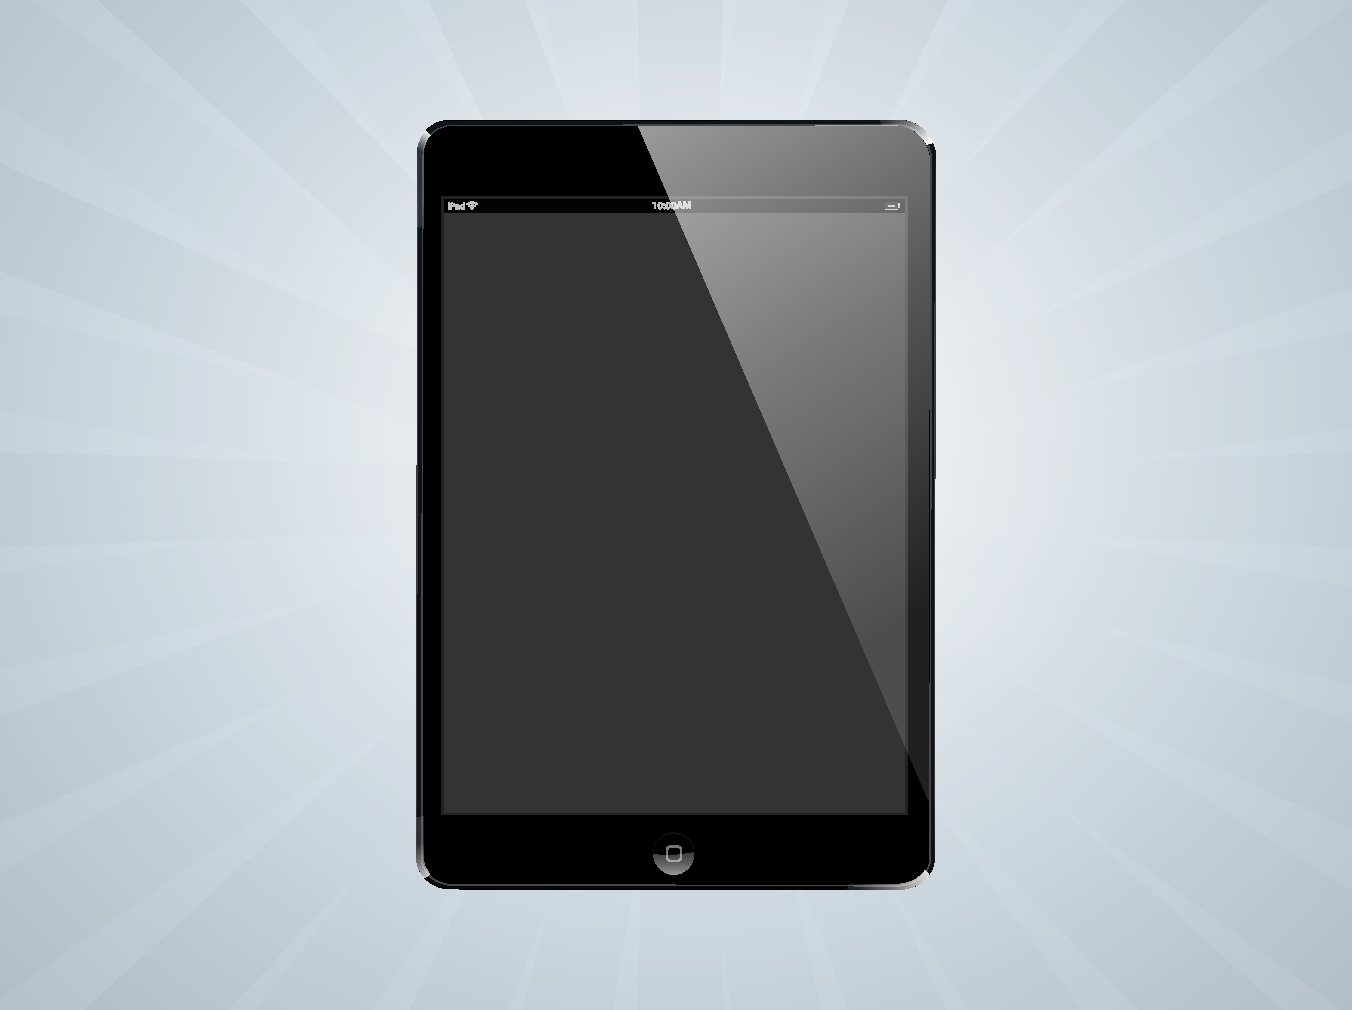
\includegraphics[width=8cm]{ipad.pdf}
	\caption{Vektorový obrázek iPadu mini}
	\label{ipad}
\end{figure}

\newpage

\section{Zdrojový kód}

\lstinputlisting[language=PHP]{source.php}

\newpage

\begin{thebibliography}{9}
	\bibitem{latex}
		KOPKA, Helmut; DALY, Patrick W.
		\textit{Latex kompletní průvodce},
		1. vydání,
		Brno: Computer Press, 2004,
		s. 584,
		ISBN: 80-722-6973-9.
	\bibitem{jreichl}
		\textit{Galileo Galilei} [online].
		Wikipedia: the free encyclopedia. San Francisco (CA): Wikimedia Foundation, 2001-.
		Dostupný z~WWW: \url{<http://cs.wikipedia.org/wiki/Galileo_Galilei>}.
	\bibitem{ipadcite}
		\textit{Vector iPad Mini} [online],
		FreeVector.com,
		18. 09. 2013,
		[cit. 12. 06. 2014],
		obrázek ve formátu PDF.
		Dostupné z~WWW: \url{<http://www.freevector.com/vector-ipad-mini/>}.
\end{thebibliography}

\end{document}